\section{Method}

\subsection{Overview}

% 如图1所示，SparseAD由3个模块组成，分别用于实现基于稀疏query的 perception, motion forecasting 以及 decision&planning 模块组成。在Sparse AD中，query负责表征自动驾驶场景中的所有信息，并负责在不同模块中实现信息的传递与交互和梯度端到端优化。与之前的方法不同，本方法并不以来稠密的BEV特征，其避免其带来的显著计算和显存负担。多相机图像在经过特征提取器后，通过3D PE后，被输入到感知模块中，这些原始传感器信息将被聚合到多种query中（detection, tracking, mapping query）作为对驾驶场景的稀疏表征在下游任务中传递。 
% 特别的，本方法提出了提出了一种端到端的多任务memory bank, 用于统一存储整个驾驶场景的时序信息，提供给端到端AD中的不同任务使用。我们将所存储的时序信息根据对象分为三个级别，scene-level, instance-level和ego-level。其中scene-level以frame为单位记录时序信息，其中包含历史帧场景内的障碍物（det query）和地图（map query）时序信息。Instanse-level记录了被追踪对象的时序信息，每个instance内包括了其在历史帧中的跟踪信息(track query)和行为预测信息（forecasting query）。Ego-level记录了自车的时序信息，包括历史帧中所做出的决策（decision query）和规划(planning query)以及command。所提出的e2e多任务memory back遵循FIFO原则，特别的，当一个instance从场景中消失一定时间后，其所有的历史信息将会被从memory中全部移除。
%
As shown in \cref{fig:arch}, \model comprises three sparse query-based modules for perception, motion forecasting, and decision \& planning respectively. In Sparse AD, queries are responsible for representing all the information in the driving scenario, transferring and interacting information across modules, and propagating backward gradients for optimization in multi-tasks in an end-to-end manner. Different from previous methods\cite{hu2023planning}, \model does need the view-projector\cite{philion2020lift} and dense BEV features, which avoids the heavy computational and memory burden\cite{liu2022petr,jiang2023far3d, zhang2023fully}. The perspective-view features for multi-camera images are extracted by a shared backbone and are fed into the perception module with 3D PE\cite{liu2022petr}. These raw sensor information will be aggregated into multiple kinds of query (detection, tracking, mapping query) as a sparse representation of the driving scenario to be passed in the full-stack tasks.

Specifically, an end-to-end multi-task memory bank is introduced in this paper for uniformly storing the temporal information of the entire driving scenario, which makes it feasible to benefit from temporal information for full-stack tasks in the end-to-end AD. We categorize the stored temporal information into three levels: scene-level, instance-level, and ego-level. The scene-level memory stores the temporal information as frames, which contain the obstacles (detection queries) and map elements (map queries) within the driving scenario in history frames. Instance-level memory serves for the tracked object, which includes the track query and forecasting query in the history frames for each instance. Ego-level records the temporal information of the ego-vehicle, which includes the history decision (decision query), and planning (planning query) command. The proposed end-to-end multi-task memory follows the FIFO (First Input First Output) principle. In particular, when an instance disappears from the scene for a period of time, the instance with all of its history information will be removed from memory.


\subsection{Perception}

\begin{figure}[tb]
  \centering
  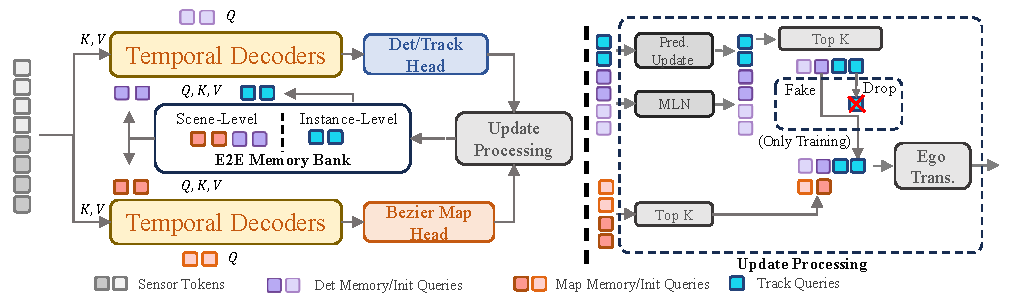
\includegraphics[width=1\linewidth]{Figures/Det-Map-Arch-Figure}
  \caption{\textbf{稀疏感知}模块，由两个统一解码器和两个对应的头部分别用于检测\&跟踪和在线建图。}
  \label{fig:dt-map-arch}
\end{figure}

% 如图三所示，parseAD的感知模块由检测跟踪子模块和地图子模块构成，两者具有相似的模型设计。本节中我们将分别对这两个子模块进行介绍。
As shown in \cref{fig:dt-map-arch}, the perception module of SparseAD consists of a detection tracking sub-module and an online mapping sub-module, both of which have similar model designs. In this section, we will introduce these two submodules separately.

% 我们的检测追踪模块联合进行检测和多物体跟踪任务，并且无需额外的后处理。之前已经有很多工作实现了端到端的MOT，其一般使用track query与gt建立绑定关系，并将track query与关联的gt一起帧间进行传递和监督。然而，这种方式使得track query获得良好的端到端特性的同时，也使得模型的检测性能出现大幅退化。

\subsubsection{Detection\&Tracking}. This module jointly performs detection and MOT(multi-object tracking) tasks without any additional post-processing. End-to-End MOT paradigm has been studied by some previous works\cite{zeng2022motr,yu2023motrv3, pang2023standing, gu2023vip3d, hu2023planning}, which use track queries to establish association relationships with ground-truth bounding boxes, which are propagated and supervised together frame-by-frame. Although this paradigm brings end-to-end tracking characteristics to track queries, which is what we are happy to see, it causes a significant degradation in the detection performance of the model\cite{yu2023motrv3, hu2023planning}.

% 为了解决这个问题，我们提出了两个方法来缓解这个问题: 1、我们设计了一种 two-level memory架构，在帧间同时使用不和gt绑定的frame-level memory和与gt绑定的instance-level memory。以确保更多的历史帧信息可以被有效的利用（比如低分TP），并确保历史帧的信息不会随着某个instance的消失而完全消失。对two-level的query，我们使用不同的更新方法，前者使用速度，后者使用预测轨迹，使得treackquery可以更充分的利用instance-level的信息。2、具有高置信度的query会同时被存储进两个level的memory并传递到下一帧，使模型难以区分。对此，我们设计了一种trackquery的增广方式，在memory向下一帧传递时加入额外相似的的fp instance，以提升模型区分trackquery与detquery的能力，减少潜在的id switch风险。并在训练中对帧间传递的trackquery随机丢弃，以解绑其与gt的绑定关系，以保证det query也具有充分的监督。


In this module, We propose two ways to mitigate this problem: 1. We design a two-level memory framework for the end-to-end MOT task, which uses both frame-level memory and instance-level memory to propagate temporal information across frames, where the latter has associations with the ground truths across frames and the former does not. The framework ensures that all temporal information of history can be effectively utilized (e.g., low-scoring TP), and prevent the information loss from removed instance memory when an instance dies. The scene-level memory is updated by the velocity prediction across frames and the instance-level memory is updated by the instance motion forecasting from the downstream forecasting task to fully utilize instance-level temporal information. 2. Queries with high confidence are simultaneously stored in both levels of memory and propagated to the next frame, making it difficult for the model to differentiate between them in the next frame. To alleviate this problem, we design a track query augmentation method, which adds similar FP instances to the instance-level memory when propagating frame-by-frame to force the model to distinguish track queries and detection queries, further reducing the potential of id switches. The track queries are randomly dropped during training simultaneously which releases the ground truth to ensure sufficient supervision of detection queries.

% 拟议的检测和跟踪模块如图 2 所示。为了进一步提高效率，我们使用了额外的 2D RoI head 来过滤前景标记。整个解码器由 N 层组成。每一层中的查询和场景级内存首先由 MLN 进行投影并与 HybirdAttention 进行交互，然后与 3DPE 嵌入的透视图像特征进行交互。最后由该模块输出 3D 检测和 MOT 结果。根据输出查询的置信度得分，查询结果将存储在不同级别的存储器中，供下游任务和未来帧使用。


The proposed detection \& tracking module is shown in \cref{fig:dt-arch}. To further improve the efficiency, we use an additional 2D RoI head to filter foreground tokens\cite{wang2023focal}. The whole decoder is composed of N layers. The queries and scene-level memory in each layer are first projected by MLN and interact with Hybird-Attention\cite{wang2023exploring}, then interact with the perspective-view image features embedded by 3D-PE\cite{liu2022petr}. 3D detection and MOT results are output by this module finally. Depending on the confidence score, the queries will be stored in different levels of memory for downstream tasks and future frames.

%注;关于多模态的内容忘记加载描述和图片里了，这块之后还需补充一下。
%注： 这里可能后续会和detection & tracking一起合并称为 preceptron模块，使得整体架构更加简洁。这也是由于map的范式确实和detection比较相似。因此，这里的图的链接也先指向了det的图，之后两个图会合二为一（现在还没画）。 注：已经完成

% 地图信息为轨迹预测和自车规划提供了很强的先验信息，是自动驾驶任务不可缺少的一环。近年来对于Online mapping的研究已经取得显著的进展，与检测任务类似，在Mapping任务上引入时序也为模型的性能带来显著提升。然而，现有的方法都需要依赖bev特征，使得拓展现有地图模型的检测范围（60m x 30m）至与其他自驾任务一致(100m x 100m)需要付出很高的成本。

\subsubsection{Online Mapping}. Map provides strong prior information for motion forecasting and ego planning, which is an indispensable part of autonomous driving. Online mapping has received more and more attention in recent years\cite{li2022hdmapnet,liu2023vectormapnet,qiao2023end,ding2023pivotnet}. Similar to the detection task, this task also benefits from the introduction of temporal information\cite{yuan2024streammapnet}. However,  to the best of our knowledge, all of the existing methods rely on BEV features, making it nontrivial to extend the detection range of the existing map method ($60m \times 30m$) to be consistent with other self-driving tasks ($100m \times 100m$) since the high memory and computational cost.

% 针对这个问题，我们提出一种稀疏的时序地图模块，如图1所示。其具有和检测跟踪模块近似的结构。具有先验类别的稀疏query被均匀散布在XY平面上，并通过3DPE与图像特征进行交互。与检测模块不同，我们使用Piecewise B´ezier Output Head用于对地图元素的回归。我们所提出的架构将地图和检测追踪任务统一为类似的分类-回归任务，并使用相似的模型结构进行处理，极大的多任务的Pipeline。注意到，地图任务对模型感受野的要求和检测追踪任务具有较大的差异，但受益于我们所使用的的全局注意力算子所提供的全局感受野，我们并不需要额外使用复杂的算子来适应地图任务对感受野的需求。

To address this problem, we propose a sparse stream map module as shown in Fig. 1. It has a similar paradigm to the detection \& tracking module. The sparse query with a priori class is uniformly scattered in the XY plane and interacts with the image features via 3DPE\cite{liu2022petr,yan2023cross} and attention modules. Difference from the detection module, we use the Piecewise Bezier Output Head\cite{qiao2023end} to regression the piecewise bezier curve of map elements. The proposed architecture unifies the map and detection-tracking tasks into similar classification-regression tasks and processes by similar modules, which greatly concurs with the complexity of the end-to-end multi-task pipeline. Note that the perception of map elements requires a larger receptive field compared with the detection-tracking task due to the various shapes of the map elements\cite{yuan2024streammapnet}. However, thanks to the global receptive fields provided by the global attention operator\cite{vaswani2017attention} used in our paradigm, there is no need to use additional complex operators to accommodate the receptive field requirement of perception of map elements.

\subsection{Motion forecasting \& Planning}

%这里参考了songnan投稿cvpr2024的论文，应该需要引用一下。但是他现在还没在arxiv上挂出来，等论文公开之后可以加以引用。

%最近已经有很多研究将transformer结构应用在prediction模块中并取得了出色的性能。为了贯彻我们所提出的sparse query-centric精神，我们这里也提出一种基于transofrmer的行为预测模块。预测模块所需要的所有驾驶场景信息均被被存储在我们所提出的端到端多任务memory bank，包括历史的agent预测表征，和当前时刻的agent表征以及地图表征，并以高度抽象的稀疏query形式表达。最终，本模块会预测所有agent的未来K个可能的轨迹。类似于Motionformer，本方法是一个在一次前向计算中产生多agent 轨迹预测，大幅降低了模型的计算成本。

\input{Figures/Fore-Arch.tex}

Recently there has been a lot of research implementing the transformer architect in the motion forecasting task and achieving excellent performance\cite{zhou2022hivt,gao2020vectornet,chai2019multipath,zhang2023real,ngiam2021scene,zhou2023query}. Following the spirit of sparse query-centric, we also propose here a motion forecasting module based on transformers. All the information about the driving scenario required by the module is stored in the proposed end-to-end multi-task memory bank, including temporal agent prediction representations, current and temporal agent representations, map representations, etc., in the form of highly abstract sparse queries. Finally, this module predicts the top K possible future trajectories of all agents. Similar to Motionformer\cite{hu2023planning,shi2022motion}, the present approach produces multi-agent trajectory predictions in a single forward pass, which reduces the computational cost of the module.

% 如图所示所提出的预测模块由一个历史聚合模块和为N层交互模块组成。其中交互模块模块由四个子模块串联而成，分别负责 modal-modal, agent-memory ,agent-agent, agent-map四个维度上的信息交互。历史聚合模块主要聚合agent-level的历史信息，包括历史位置和历史track query，为预测query提供先验信息。历史聚合模块分别在polyline和query两个维度上进行聚合，所示。

The proposed forecasting module as shown in \cref{fig:fore-arch}, consists of a history aggregation module and for N-layer interaction module. The interaction module consists of four sub-modules, which are responsible for the information interaction in four dimensions: modal-modal, agent-memory, agent-agent, and agent-map. The history aggregation module aggregates the history information at the agent level, including temporal location and temporal track queries, and aims to provide a priori information for the multi-modal forecasting queries. The history aggregation module aggregates on polyline and query dimensions successively as shown in \cref{eq:his_aggreation}.

\begin{equation}
  Q_A^i = \text{MHCA}(P^i, \mathcal{Q}_{MT}^i)
  \label{eq:his_aggreation}
\end{equation}
where
\begin{equation}
  P^i = \text{G}(\mathcal{P}^i)
  \label{eq:his_aggreation}
\end{equation}
% QA_i = MHCA(P_i, T_i)
% 其中， P_i = G(V_i) P是Polyline level的Feature。V_i是 agent i的历史轨迹向量。
where $Q_A$ donate multi-modal forecasting queries, $i$ is the index of the agent, MHCA donates the multi-head cross-attention, $\mathcal{Q}_{MT}^i$ and $\mathcal{P}^i$ is the set of temporal memory track queries and temporal trajectory vectors of agent $i$,  $P^i$ is the polyline representation of $\mathcal{P}^i$, and $\text{G}$ is the sub-graph encoder\cite{gao2020vectornet}. 

%交互模块进行agent在模态维度的交互和与驾驶场景的交互，其中的多个交互依次进行。其中，modal-modal interaction可以表示为公式3，agent-memory, agent-agent, agent-map的交互可以表示为公式4。
The interaction module performs the interaction of agents in the modal dimension and with the driving scene, where multiple interactions are performed sequentially. The modal-modal interaction and the agent-memory, agent-agent, and agent-map interactions can be represented as \cref{eq:modal_interaction} and \cref{eq:scene_interaction} respectively.

\begin{equation}
  Q_A^i = \text{MHSA}(Q_A^i)
  \label{eq:modal_interaction}
\end{equation}

\begin{equation}
  Q_A^i = \text{MHCA}(P^i, \mathcal{Q}_{MF}^i / \mathcal{Q}_M / \mathcal{Q}_T)
  \label{eq:scene_interaction}
\end{equation}
%其中....（符号解释）... 
where $\mathcal{Q}_{MF}^i, \mathcal{Q}_M, \mathcal{Q}_T$ donate the set of temporal memory forecasting queries of agent $i$, the set of the map queries in the current scene, and the set of track queries in the current scene. 

% 特别的，我们为不同任务设计了不同的位置嵌入。对于forecasting memory，这里提出 Time Stamp Align Trajectory Positon Embedding，用于编码当前帧与历史帧预测的一致性。为了简化描述，这里忽略了模态序号m。Agent i 在T时刻对未来N帧的轨迹预测可以表示为...，forecasting memory存储的预测轨迹则可以表示为...，其中N为memory的长度。这里我们认为历史轨迹已经被转换到了当前时刻的自车坐标系下。

We propose several positional embeddings for different interactions. For agent-memory interaction, Timestamp-Aligned Trajectory Position Embedding is proposed to encode the consistency between temporal motion forecasting. To simplify the description, the modal order $m$ is ignored here. the motion prediction of agent $i$ for the future M steps at time T can be expressed as  ${\cal F}_T^i = \{ {{\bf{v}}_{\bf{1}}},...,{{\bf{v}}_M}\}$, The historical forecasting trajectory in memory can then be expressed as $\left\{ {{\cal F}_{T - 1}^i,...,{\cal F}_{T - N}^i} \right\}$,  where $N$ is the length of memory. To simplify the problem, we assume that the temporal forecasting trajectories have been transformed into the current ego-car coordinate system. Timestamp-aligned trajectory position embedding of agent $i$ for forecasting memory $E_{FM}^i$ and current forecasting $E_{FA}^i$ can be expressed as \cref{eq:ts_align_pe_memory} and \cref{eq:ts_align_pe_agent} respectively 
\begin{equation}
    E_{FM}^i = \sum\limits_{k = 1}^N {{\rm{ML}}{{\rm{P}}_k}({\rm{Cat}}(\{ {{\bf{v}}_j} - {{\bf{v}}_k}|j \ge k,{\bf{v}} \in {\cal F}_{T - k}^i\} ))} 
    \label{eq:ts_align_pe_memory}
\end{equation}

\begin{equation}
    E_{FA}^i = \sum\limits_{k = 1}^N {{\rm{ML}}{{\rm{P}}_k}({\rm{Cat}}(\{ {{\bf{v}}_j} - {{\bf{v}}_0}|j \le M - k,{\bf{v}} \in {\cal F}_T^i\} ))} 
    \label{eq:ts_align_pe_agent}
\end{equation}

%对于agent-agent的交互，我们根据agent的空间位置进行3DPE。对于agent-map的交互，我们提出curve pe，使用一系列空间采样点作为位置编码。根据感知模块所预测出的贝塞尔系数c，我们以可忽略的成本实现对地图曲线的进行采样，其中，n是贝塞尔曲线的阶数。
For agent-agent interaction, we perform 3DPE\cite{liu2022petr,yan2023cross} based on the spatial locations of agents. For agent-map interaction, we propose Curve Position Embedding, which encodes a series of spatially sampled points as the embedding. Based on the Bezier coefficients $c$ predicted by the perception module, we sample $J$ points $\mathcal{C}_M = \{\bf{p}_1,...,\bf{p}_J\}$ on the curve of map elements with a negligible cost as shown in \cref{eq:bezier_eq_1} and \cref{eq:bezier_eq_2}, where n is the order of the Bezier curve.
\begin{equation}
p(t)=\sum_{i=0}^n b_{i, n}(t) c_i, t \in[0,1]
\label{eq:bezier_eq_1}
\end{equation}
where
\begin{equation}
b_{i, n}(t)=\left(\begin{array}{c}
n \\
i
\end{array}\right) t^i(1-t)^{n-i}, i=0, \ldots, n
\label{eq:bezier_eq_2}
\end{equation}

% 类似的，可以通过agent的位置向量$\bf{p}_A$ J次形成一个伪曲线 $\mathcal{C}_A = \{\bf{p}_A,...,\bf{p}_A\}, CurePE可以表示如下
Similarly, a pseudo-curve $\mathcal{C}_A = \{\bf{p}_A,...,\bf{p}_A\}$ can be formed by repeat the agent's position vector $\bf{p}_A$ $J$ times. Curve PE can be expressed as follows

\begin{equation}
    E_{C} = \sum\limits_{k = 1}^J {{\rm{ML}}{{\rm{P}}}({\rm{Cat}}(\{ {{\bf{p}}_j}|{\bf{p}} \in {\cal C}\} ))} 
    \label{eq:ts_align_pe_agent}
\end{equation}

%最终，预测模块所产生对multi-agent的top k轨迹预测将被存储至端到端多任务memory bank中，以供planning模块使用。这些轨迹预测也会用于在帧间更新instance-level memory 中的 先验position信息。
Finally, the Top k trajectory predictions for multi-agents generated by the prediction module will be stored in the end-to-end multi-task memory bank for the downstream planning module. These trajectory predictions are also used to update the priori position information of instance-level memory across frames.

\subsection{Planning}
% For Planning，我们在ego-level而非scene-level上考虑了planning的时序性。具体而言，我们在planning中融入流式的思想，再下一次预测planning轨迹时会同时结合历史的预测结果和环境信息。我们的planning模块和上游任务都是基于transformer架构进行设计，并以parse query-centric为中心思想设计模块。在和障碍物的交互过程中，ego queries同时结合了跟踪和多模态预测这两个不同level的abstract sparse queries，在做planning任务的同时，我们对障碍物对ego的阻挡关系进行预测，我们发现加入这一个辅助任务可以使ego更加attention到重要障碍物信息。在Sec. \ref{}中展示这一辅助任务对模型的提升。在地图的交互中，为了使ego queries充分感知到有效地图信息，交互的地图queries只会集中于与自车相邻的地图线，在交互中还设计了大量约束来强化ego queries对地图的有效信息感知。

For Planning, we focus on the temporal aspects of planning at the ego-level rather than at the scene-level. Specifically, our approach integrates a streaming concept within the planning process, where the prediction of future trajectories simultaneously incorporates both historical outcomes and contextual environmental data. Our planning module, along with upstream tasks, is designed based on the transformer architecture, adopting 'parse query-centric' as the core design principle. During interactions with obstacles, ego queries amalgamate tracking and multimodal prediction, representing two distinct levels of abstract sparse queries. While undertaking planning tasks, we also predict the obstructive relationships between obstacles and the vehicle of the ego. We found that incorporating this auxiliary task significantly enhances the ego's focus on critical obstacle information, as demonstrated in Section \ref{}. In terms of map interaction, to ensure that ego queries adequately perceive relevant map information, the interacting map queries are concentrated around road lines adjacent to the autonomous vehicle. Additionally, we designed numerous constraints to reinforce the ego queries' effective perception of map information.

% The proposed planning module as shown in Fig. \ref{},planning head按照功能可以大致被划分为四个stage，每个阶段都在本节中展开叙述。

\subsubsection{Ego-Queries Init}
% 在Ego-Queries Init过程中，planning会从memory-bank中找到上一时刻存储的ego query作为一个history query ($\mathcal{Q}_{ego}^{memory}$)，同时从自车传感器等信息初始化另一个action query ($\mathcal{Q}_{ego}^{action}$)，使模型兼顾历史预测信息和ego瞬时状态信息，生成出满足控制约束的稳定planning轨迹。为了表达ego和障碍物之间的相对位置关系，同样对ego queries加入了位置编码，虽然ego在lidar系下始终静止。为了更清晰阐述方法，这两个queries用集合$\mathcal{Q}_{ego}$表示：
\begin{align}
  \mathcal{Q}_{ego} &= \{Q_{ego}^{memory}, Q_{ego}^{action}\} \\
\end{align}

\subsubsection{Ego-Agent Interaction}
% ego agent的交互可以被描述为：
\begin{align}
  \mathcal{Q}^{lvl-1}_{ego} &= \text{MHCA}(\mathcal{Q}_{ego}, \mathcal{Q}_{MT} / \mathcal{Q}_{MF}) \\
  % \mathcal{Q}^{lvl-2}_{ego} &= \text{MHCA}(\mathcal{Q}_{ego}^{lvl-1}, \mathcal{Q}_{MF}) \\
  \mathcal{Q}_{AD} &= \text{MHCA}(\mathcal{Q}_{MF}, \mathcal{Q}_{ego}^{lvl-1}) \label{eq:agent_decision}\\
  \mathcal{Q}^{lvl-2}_{ego} &= \text{MHCA}(\mathcal{Q}_{ego}^{lvl-1}, \mathcal{Q}_{{AD}})
\end{align}
% 其中$\mathcal{Q}_{MT}$是从memory bank中取出的跟踪feature，$\mathcal{Q}_{MF}$是从memory bank中取出的预测feature，Eq. \ref{eq:agent_decision}是引入的额外辅助任务，隐式的让模型学习那些障碍物是重要障碍物，在和跟踪预测的feature交互后，再用预测的feature和ego features交互一次，得到agents decision($\mathcal{Q}_{AD}$)集合，集合元素数和障碍物数量相同。对$\mathcal{Q}_{AD}$Sec. \ref{sec:planning_constrains}中阐述。最后$\mathcal{Q}_{ego}$ 再和 $\mathcal{Q}_{AD}$ 做一次cross-attn完成agent和障碍物之间的交互。

\subsubsection{Ego-Map Interaction}
% Planning模块对地图的处理与预测一致，同样使用Curve Position Embedding as shown in \cref{eq:bezier_eq_1} and \cref{eq:bezier_eq_2}。
\begin{align}
  \mathcal{Q}^{lvl-3}_{ego} &= \text{MHCA}(\mathcal{Q}^{lvl-2}_{ego}, \mathcal{P})
\end{align}

\subsubsection{Ego Planning Head}
\label{sec:planning_head}
% $\mathcal{Q}_{ego}$在与障碍物和地图交互后，SparseAD使用一个简单的MLP模型将$\mathcal{Q}_{ego}^{history}$和$\mathcal{Q}_{ego}^{action}$进行融合：
\begin{equation}
    Q_{ego}^{memory} = \textrm{MLP}(\mathcal{Q}_{ego}^{lvl-2}, \mathcal{Q}_{ego}^{lvl-3})
\end{equation}

% $\mathcal{Q}_{ego}^{memory}$存放在memory bank中，供下次planning使用。对融合后的feature再解码成future waypoints $\hat{\tau}$ ，得到ego的路径规划:
\begin{equation}
    \hat{\tau} = \textrm{MLP}(Q_{ego}^{memory})
\end{equation}

\subsubsection{Planning Constrains}
\label{sec:planning_constrains}
% 在ego query和障碍物与地图的交互过程中，SparseAD设置了多样的约束监督模型学习。除了几种常见的Ego-Lane and Ego-Agent Loss (我们在附录中详细介绍他们)，SparseAD还引入了Ego-Agent Decision Loss来对障碍物和自车的阻挡关系进行额外的辅助任务监督。
% 具体而言，遵循着大多数工作\ref{}，我们使用rule-base的方法结合障碍物和自车的未来轨迹，生成障碍物在自车行进方向和垂直自车行进方向上的阻碍关系，沿自车行进方向生成标签{前向阻碍，后向阻碍，无阻碍}，垂直自车行进方向生成标签{左向阻碍，后向阻碍，无阻碍}对 Eq. \ref{eq:agent_decision}中的$\mathcal{Q}_{{AD}$，对其分别解码出在不同方向上的阻挡关系：
\begin{align}
    \hat{\mathcal{D}^H} &= \textrm{MLP}(Q_{AD}) \\
     \hat{\mathcal{D}^V} &= \textrm{MLP}(Q_{AD})
\end{align}
% where $\hat{\mathcal{D}^H}$是垂直自车行进方向上的预测结果，$\hat{\mathcal{D}^V}$是沿着自车行进方向上的预测结果。

% 之后使用focal loss监督，这一项Ego-Agent Decision Loss (\mathcal{L}_{AD})可以表示如下：
\begin{equation}
    \mathcal{L}_{AD} = - \sum_{i=1}^A\sum_{j=1}^C\alpha_i(1-\hat{D^H_{ij}})^\gamma \log \hat{D^H_{ij}} - \sum_{i=1}^A\sum_{j=1}^C\alpha_i(1-\hat{D^V_{ij}})^\gamma \log \hat{D^V_{ij}}
\end{equation}
% where $A$是障碍物数量，$C$是类别数目，$\alpha_i$是为了平衡样本分布所设置的参数。这里我们将$\alpha$设置成{xx,xx,xx}。其中i=0时对应无阻碍。


